%----------------------------------------------------------------------------------------------------------------------

\documentclass[a4paper,12pt]{report}
\usepackage[utf8]{inputenc}
\usepackage[portuguese]{babel}
\usepackage{graphicx}
\usepackage{hyperref}
\usepackage{float}
\usepackage{listings}
\usepackage{longtable}
\usepackage{subfig}
\usepackage{tabularx}
\usepackage[table,xcdraw]{xcolor}
\usepackage{adjustbox}
\newcommand*{\xml}[1]{\texttt{<#1>}}
\usepackage[T1]{fontenc}
\usepackage{lmodern}
\newcommand*{\escape}[1]{\texttt{\textbackslash#1}}
\newcommand*{\escapeI}[1]{\texttt{\expandafter\string\csname #1\endcsname}}
\newcommand*{\escapeII}[1]{\texttt{\char`\\#1}}

%----------------------------------------------------------------------------------------------------------------------

\usepackage{geometry}
 \geometry{
     a4paper,
     total={170mm,257mm},
     left=25mm,
     right=25mm,
     top=20mm,
 }

\graphicspath{{./base_images/}}

%----------------------------------------------------------------------------------------------------------------------

\begin{document}

%----------------------------------------------------------------------------------------------------------------------


\begin{titlepage}
    \center
    {

    \begin{figure}[t]
        \centering
        
\includegraphics[scale=0.4]{images/uminho.png}
        \label{img:logo}
        \vspace{2.0cm}
    \end{figure}

    \vspace{3.0cm}
    \textsc{\Huge Processamento de Linguagens}\\[0.5cm]
    \textsc{\Large{Mestrado Integrado em Engenharia Informática}}\\[0.5cm]
    \vspace{3cm}
    \textsc{\textbf{\Huge{Trabalho Prático nº 1}}}\\[1cm]
    \textsc{\huge{FLex}}\\[1cm]
    \vspace{4cm}
    \begin{flushleft}

        \vspace{1cm}
        \large Grupo XX
        \vspace{0.5cm}

        \large A85227 \,\,\,João Pedro Rodrigues Azevedo
        \vspace{0.2cm}

        A85729 \,\,\,Paulo Jorge da Silva Araújo
        \vspace{0.2cm}

        A83719 \,\,\,Pedro Filipe Costa Machado
        \vspace{0.2cm}

    \end{flushleft}
    \begin{flushright}
        Braga

        Abril 2020
    \end{flushright}

\date{\today}
}
\end{titlepage}

%Indice

\tableofcontents
\clearpage

% Introdução

\chapter{Introdução}

Este relatório é relativo ao trabalho prático da UC de Processamento de Linguagens que tem como um dos principais objetivos desenvolver, a partir de \textit{Expressões Regulares (ER)} e processadores de linguagens regulares capazes de alterarem e transformarem textos através do conceito de regras de produção Condição-Ação. 

Para tal, iremos recorrer ao \textit{FLex} para gerar filtros de texto em C, num ambiente de trabalho \textit{Linux} e outras ferramentas de apoio. 

Assim, iremos analisar ficheiros de texto e tentar encontrar padrões de frases nos mesmos, de forma a ser possível criar \textit{ERs}, que depois irão reagir da forma que nós estipulamos às mesmas, criando os resultados esperados.


\chapter{Enunciado Escolhido}

Com vista a realizar este trabalho, foram-nos propostos pela equipa docente seis enunciados e pedido, pela mesma, para escolhermos um. 
\par Depois de algum debate entre os membros do grupo, achamos por bem escolher o \textbf{TransformadorPublico2NetLang} (enunciado 4). Neste enunciado, era nos pedido que analisássemos um ficheiro \textit{HTML} que continha 85 comentários extraídos de uma notícia publicada na versão online do jornal "O Público". 

Com a finalidade de se fazer um estudo sócio-linguístico de forma e conteúdo dos comentários que a notícia suscitou, era pretendido extrair do ficheiro \textit{HTML} a informação relevante para análise. 

De seguida, pedia-se que transformasse-mos esta informação para um formato \textit{JSON}, como indica a figura \ref{img:Json_Struct}.

\begin{figure}[h]
        \centering
        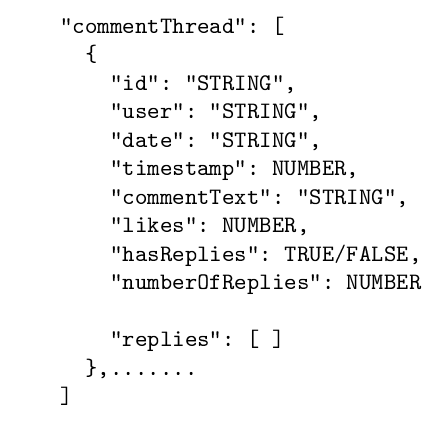
\includegraphics[scale=0.5]{images/jsonStruct.png}
        \caption{Formato Json}
        \label{img:Json_Struct}
        \vspace{2.0cm}
    \end{figure}

Esta escolha deveu-se ao facto de ser desafiante a procura de padrões num ficheiro de texto e ainda ser necessário a utilização de uma estrutura que consiga armazenar estes mesmo padrões em memória, para posteriormente serem utilizados com a sua respetiva finalidade.


\chapter{Estratégia Adotada}

Numa primeira fase, o grupo começou por analisar os comentários da página de notícias do jornal através do \textit{browser} de Internet, tirando notas relativas ao tipo de comentários que poderiam existir. A título de exemplo, o grupo notou que os utilizadores podiam possuir caracteres especiais na sua identificação (nome de \textit{user}).

De seguida, obtivemos o ficheiro \textit{HTML} a partir do comando Linux \textit{wget}, podendo começar, assim, uma análise mais detalhada ao modo do qual os comentários estavam estruturados.
\par Neste capítulo, iremos abordar a estrutura do ficheiro \textit{HTML} em que trabalhamos, bem como a nossa implementação e especificação do filtro \textit{FLex}.

\vspace{1 cm}

\section{Estrutura do Ficheiro HTML}

\vspace{0.5cm}

O ficheiro \textit{HTML} possui várias \textit{tags} que o grupo definiu como relevantes no que conta à recolha de informação e, posteriormente, à definição de \textit{ERs}. Assim, iremos indicar quais \textit{tags} o grupo teve especial atenção e explicar qual o seu propósito.

\begin{itemize}
    \item 
    \xml{ol}
    \par Esta \textit{tag} indica que até ao final desta (\xml{/ol}) estariam um conjunto de comentários, representados pela \textit{tag} \xml{li}. De realçar que o ficheiro \textit{HTML} possui uma \xml{ol} principal que contém todos os comentários principais. Esta \textit{tag} é representada por ter como etiqueta de abertura os atributos "\textit{class}" e "\textit{id}", como se segue no exemplo:
    
\begin{center}
    \begin{lstlisting}[language = html]
<ol class="comments__list" id="approved-comments">
..
</ol>
    \end{lstlisting}    
\end{center}   

    Juntamente a este uso da \textit{tag}, esta pode também representar uma lista de \textit{replies} a um dado comentário. Este tipo de utilização da \textit{tag} é identificável por apenas possuir o atributo "\textit{class}", como se observa no seguinte exemplo:
    
\begin{center}
    \begin{lstlisting}[language = html]
<ol class="comments__list">
..
</ol>
    \end{lstlisting}    
\end{center}   
\end{itemize}

\vspace{1cm}

\begin{itemize}
    \item 
    \xml{li}
    \par A \textit{tag} \xml{li} serve para guardar todas as informações de um comentário. Dentro desta, podemos encontrar uma \textit{tag} \xml{div}, que contém outras duas \textit{tags} \xml{div}, cada uma contendo informações diferentes, ou seja a "\textit{meta}" ou o "\textit{content}" do comentário em causa.
    \par De realçar que dentro das \xml{div}'s existem outras \textit{tags} tais como: \xml{h5}, \xml{time}, \xml{p} e, possivelmente \xml{ol}, caso o respetivo comentário tenha \textit{replies}. 
    \par O grupo decidiu focar-se mais nestas últimas \textit{tags}, pois são mais concretas em relação à informação que se pretende obter. 
    \par Referir que \xml{li} tem uma outra \textit{tag}(\xml{form}) que o grupo não notou grande importância para a formulação do ficheiro \textit{Json}. 
    Um exemplo do uso desta \textit{tag} é o seguinte:
    
    \begin{center}
\begin{lstlisting}[language = html]
<li class="comment" data-comment-id="06..">
    <div class="comment__inner">
        <div class="comment__meta">..</div>
        <div class="comment__content">..</div>
    </div>
    ..
</li>
    \end{lstlisting}    
\end{center} 
    Neste exemplo, verificámos que o valor do atributo "\textit{data-comment-id}" representa o \textit{id   } do comentário.
\end{itemize}

\vspace{0.4cm}

\begin{itemize}
    \item 
    \xml{h5}
    \par Com o \xml{h5} e, dentro desta a \textit{tag} \xml{a}, podemos obter o nome do utilizador responsável pelo comentário. Esta \textit{tag} é a primeira dentro de um \xml{li} que se demonstra fulcral para obter a informação de forma a construir o ficheiro \textit{Json} pretendido.
    \par Segue-se de seguida um exemplo desta \textit{tag}:
    
        \begin{center}
\begin{lstlisting}[language = html]
<h5 class="comment__author">
    <a href="/utilizador/perfil/.." rel="nofollow">PdellaF </a>
</h5>
    \end{lstlisting}    
\end{center} 
    \par Assim, é possível indicar o nome do utilizador depois do caracter "\textgreater" posterior ao atributo "rel" da  \textit{tag} \xml{a}. Neste caso, o utilizador tem como nome "PdellaF".
\end{itemize}

\vspace{5cm}

\begin{itemize}
    \item 
    \xml{time}
    \par A \textit{tag} \xml{time} armazena toda a informação relativa ao momento no tempo em que a mensagem/comentário foi realizado. Dentro desta, encontra-se outra \textit{tag} (\xml{a}) na qual se encontra a data do comentário, que contém o mesmo significado que a data do \xml{time}. Assim, conseguímos obter não só a data, como também o \textit{timestamp} após alguns processamentos.
    \par De realçar que o grupo para obter os valores necessários relativos a esta \textit{tag} utilizou a data do \xml{a} como referência.
    
        \begin{center}
\begin{lstlisting}[language = html]
<time class="dateline.." datetime="2019-10-03T21:11:55.99">
    <a class="comment__permalink">03.10.2019 21:11</a>
</time>
    \end{lstlisting}    
\end{center}    
\end{itemize}

\vspace{0.4cm}

\begin{itemize}
    \item 
    \xml{p}
    \par Dentro da \xml{div} relativa ao conteúdo do comentário, encontramos a \textit{tag} \xml{p} que armazena o texto do comentário, como se observa no seguinte exemplo:
    
            \begin{center}
\begin{lstlisting}[language = html]
<div class="comment__content">
    <p>
        Como  vamos  de Salgado, Bava, Granadeiro e ..
    </p>
</div>
    \end{lstlisting}
\end{center}    
\end{itemize}

\vspace{0.4cm}

\begin{itemize}
    \item 
    \xml{h3}
    \par A \textit{tag} \xml{h3} é a primeira \textit{tag} disponibilizada pelo ficheiro \textit{HTML} e indica o número de comentários que o ficheiro possui.
    \par Embora não seja pedida para o ficheiro \textit{Json} final, a leitura desta \textit{tag} serviu para verificarmos se o nosso programa estava a ler o número correto de comentários.


          \begin{center}
\begin{lstlisting}[language = html]
<h3 class="i-comment"></i> 85 comentarios</h3>
    \end{lstlisting}
\end{center}  
\end{itemize}

\vspace{10cm}

\section{Implementação e especificação do filtro FLex}

\vspace{0.5cm}

Em primeiro lugar, o grupo desenvolveu uma estrutura de dados capaz de suportar os dados relevantes e, de certa forma, semelhante à estrutura de um \textit{commentThread} do ficheiro \textit{Json} pretendido. Assim sendo, a estrutura de dados em C, definida no ficheiro "commentThread.h" ficou da seguinte forma:


\begin{center}
\begin{lstlisting}[language = c]
typedef struct commentThread 
{
   char*        id;
   char*        user;
   char*        date;
   long int	timestamp;
   char*        commentText;
   int          likes;
   int          hasReplies;
   int          numberReplies;

   struct commentThread* next;

} *COMMENT_T;
    \end{lstlisting}
\end{center} 

\par A transformação desta estrutura para \textit{Json} é feita de maneira relativamente simples. Caso o valor "hasReplies" seja 1, ou seja, \textit{True}, então quer dizer que os próximos comentários serão \textit{replies} deste mesmo, sendo que o número de \textit{replies} é dado pelo parâmetro "numberReplies".
Assim, os comentários estão inseridos de forma ordenada em relação à leitura do ficheiro \textit{HTML}, com as respostas de cada um deles inseridas logo após o comentário principal.

\vspace{1cm}

\par De seguida, foram desenvolvidas \textbf{ERs} (Expressões Regulares) para preencher os campos da estrutura "commentThread", as quais vamos explicar de seguida o processo feito. Para tal, iremos também mostrar um diagrama para uma melhor percepção da nossa especificação do uso de \textbf{FLex} (Figura \ref{img:StateDiagramPL}).

\vspace{0.5cm}

\begin{figure}[h]
        \centering
        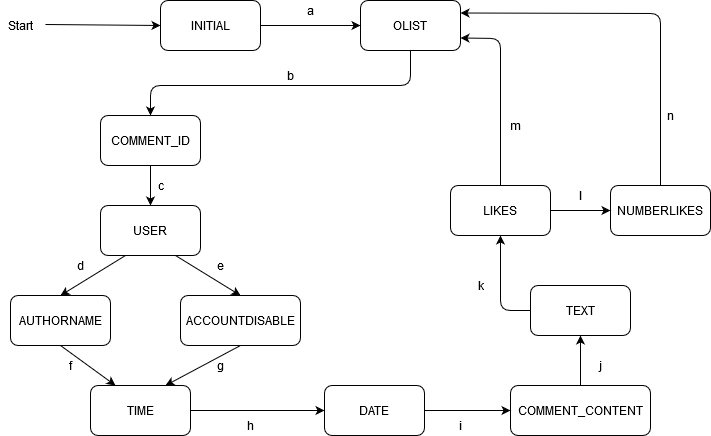
\includegraphics[scale=0.65]{images/StateDiagramPL.png}
        \caption{Diagrama de estados no FLex}
        \label{img:StateDiagramPL}
    \end{figure}


\par Este diagrama explícita como os estados definidos pelo grupo no \textit{FLex} se comportam. Assim, para cada estado e cada ligação entre eles, vamos indicar o propósito destes. De notar que as seguintes \textit{ERs} estão definidas no ficheiro "filter.l" do trabalho.  

\vspace{6cm}

\begin{itemize}
    \item 
    \textbf{Obter o número de comentários no ficheiro:}
    
    \par No diagrama observamos que o filtro começa no start e que o primeiro estado que este entra, ou seja, que dá match, é o \textbf{OLIST}. Contudo, antes de entrar neste estado o filtro executa uma \textit{ER}, sendo esta a que lê o número de comentários que estão no ficheiro.
\par Esta \textit{ER} é a seguinte:

\begin{verbatim}
    [0-9]+/[ ]+[-'a-zA-ZÀ-ÖØ-öø-ÿ]+<\/h3>\] { 
            numberComments = atoi(yytext);
            }
\end{verbatim}

\par No código acima, a ER dá \textit{match} ao conteúdo da \textit{tag} \xml{h3} que indica o número de comentários que o ficheiro \textit{HTML} possui. Segue-se um exemplo em que a \textit{ER} dá match:

\begin{verbatim}
<h3 class="i-comment"></i> 85 comentários</h3>
\end{verbatim}


Neste exemplo, depois de feito o \textit{match}, vamos trabalhar apenas com o número antes do caractere do espaço e da palavra (aceita acentos), epara isso, utilizámos a barra "/".
\par Assim, podemos armazenar o número de comentários numa variável global previamente definida, através do C, que neste caso fica a 85.

\end{itemize}

\vspace{1cm}

\begin{itemize}
    \item 
    \textbf{OLIST}
    \par O estado \textbf{OLIST} é iniciado quando há um "match" na seguinte \textit{ER}.


\begin{verbatim}
    \<ol(.*)class\=\"comments__list\"(.*)\>\< { 
        ct = (COMMENT_T) malloc(sizeof(struct commentThread));
        BEGIN OLIST; 
        }
\end{verbatim}

\par A \textit{ER} acima apenas faz "match" uma vez durante o programa inteiro (caso o ficheiro \textit{HTML} esteja na forma que esperada), pois depois de entrar neste estado o programa percorre um ciclo, como se percebe no diagrama da figura \ref{img:StateDiagramPL}. 
\par Assim, o estado \textbf{OLIST} é iniciado na \textit{tag} \xml{ol} que possui todos os comentários e é aí inicializada a estrutura de dados em C previamente referida.

\vspace{0.5cm}
\par Já no estado \textbf{OLIST}, utilizámos uma \textit{ER} para cada início de comentário (representado pela \textit{tag} \xml{li}), inicializando algumas das suas variáveis como se observa:

\begin{verbatim}
    <OLIST>li(.*)data-comment-id\=\" {  
        ct -> next = (COMMENT_T) malloc(sizeof(struct commentThread));
        ct = ct->next;

        ct->timestamp = 0;
        ct->likes = 0;
        ct->hasReplies = 0;
        ct->numberReplies = 0;

        BEGIN COMMENT_ID;
        }
\end{verbatim}

\par Após o "match", é chamado o estado \textbf{COMMENT\_ID} para trabalhar com o id do comentário.

\vspace{10cm}

\par Outra \textit{ER} definida deste estado tem como objetivo fazer "match" ao início de um conjunto \textit{replies} de um comentário, ou seja, a uma nova \textit{tag} \xml{ol}.

\begin{verbatim}
    <OLIST>\<ol(.*)\"comments__list\"\>\n*\<  {  
        ct->hasReplies = 1;
        p = ct;

        ct->next = (COMMENT_T) malloc(sizeof(struct commentThread));
        ct = ct->next;

        ct->timestamp = 0;
        ct->likes = 0;
        ct->hasReplies = 0;
        ct->numberReplies = 0;

        replies = 0;

        BEGIN COMMENT_ID;
        }
\end{verbatim}

\par Visto que estamos a trabalhar com uma \textit{reply} temos de indicar isso na estrutura de dados do comentário principal, ou seja, metemos o valor do "hasReplies" a 1. Para podermos futuramente alterar o valor "numberReplies" do comentário principal, temos de usar uma outra "commentThread" \textbf{p} para guardar os campos desse comentário.
\par De seguida, andamos com a estrutura para o próximo elemento (sendo esta agora uma \textit{reply}),  inicializar os seus valores e, por último, chamar o estado \textbf{COMMENT\_ID} para obter o seu id.

\vspace{1cm}

\par Visto que o estado \textbf{OLIST} trabalha tanto com comentários principais e as suas respostas, precisamos de uma outra \textit{ER} para verificar se as respostas de um comentário já terminaram.

\begin{verbatim}
    <OLIST>\<\/ol\>   { 
        if(countComments <= numberComments)
            p->numberReplies = replies;
        }
\end{verbatim}

\par Assim, ocorre o "match" quando encontramos o fim da \textit{tag}, ou seja, \xml{/ol}. Falta-nos apenas alterar o valor do número de respostas do comentário principal (representado pelo "p") dado pela variável definida anteriormente, "replies". Esta variável é incrementada no estado \textbf{COMMEN\_ID}.
De notar, que a condição no código serve para não meter dados errados no último comentário, quando a \textit{ER} faz "match" ao \xml{/ol} da tag principal com todos os comentários principais.

\vspace{0.5cm}

\par Por último, o programa possui uma \textit{ER} para manter o terminal limpo do texto que não deu "match" pelas \textit{ERs} definidas neste estado.
\par Esta \textit{ER} é definida várias vezes ao longo do programa e dos diferentes estados, pelo que a explicação é semelhante.
\end{itemize}

\vspace{2cm}

\begin{itemize}
    \item 
    \textbf{COMMENT\_ID}
    \par Neste estado fazemos match ao id do comentário através de uma \textit{ER} capaz de apanhar letras, números e o caracter '-', pertencentes ao id de um \textit{user}. De realçar que este estado é sempre chamado pelo \textbf{OLIST}, pelo que o match deste será sempre o id do comentário.
    
    \begin{verbatim}
        <COMMENT_ID>[A-Za-z0-9-]+/\"> {  
            replies++;
            ct->id = strdup(yytext);

            BEGIN USER; 
            }
    \end{verbatim}
    
    Para além de inicializar o id do comentário e de incrementar o número de replies, este estado também chama o estado \textbf{USER}.
    
\end{itemize}

\vspace{1cm}
\begin{itemize}
    \item 
    \textbf{USER}
    O estado \textbf{USER} tem como propósito encontrar a \textit{tag} \xml{h5}, juntamente com a \xml{a}. Com estas \textit{ERs} o objetivo é fazer match na posição correta do nome do utilizador, para permitir depois chamar o estado \textbf{AUTHORNAME} ou o estado \textbf{ACCOUNTDISABLED} possibilitando armazenar o valor do nome do \textit{user} na estrutura.
    
    \vspace{0.5cm}
    \par Caso o utilizador não tenha a conta desativada, este possui a \textit{tag} \xml{a} que contém o nome deste. Chamamos assim o estado \textbf{AUTHORNAME}.
    \begin{verbatim}
        <USER>\<h5(.*)\>\n\<a(.*)\"> { BEGIN AUTHORNAME; }
    \end{verbatim}{}
    
    \par Caso não possua a \textit{tag} \xml{a}, irá então chamar o estado \textbf{ACCOUNTDISABLED}.
    De notar que esta \textit{ER} não faz "match" a utilizadores sem a conta desativada, visto que o \textit{FLex} apanha a maior expressão, que é sempre a \textit{ER} acima.
    
        \begin{verbatim}
        <USER>\<h5(.*)\>\n[ ]+   { BEGIN ACCOUNTDISABLED; }
    \end{verbatim}{}
\end{itemize}
    
\vspace{1cm}

\begin{itemize}
    \item 
    \textbf{AUTHORNAME}
    \par A \textit{ER} deste estado faz "match" com todo o tipo de texto que vem antes do fecho das duas \textit{tags}, \xml{/a} e \xml{/h5}. Depois de obter o "match" é introduzido o valor do nome do utilizador na estrutura de dados e iniciado o estado \textbf{TIME}.
    
    \begin{verbatim}
        <AUTHORNAME>(.*)/\<\/a\>\n\<\/h5\> {
            ct->user = strdup(yytext);
            BEGIN TIME;
            }
    \end{verbatim}{}
\end{itemize}

\begin{itemize}
    \item 
    \textbf{ACCOUNTDISABLED}
    \par Este estado difere do anterior porque não possui a \textit{tag} \xml{a}, logo a \textit{ER} apenas trabalha com o conteudo que está dentro do \xml{h5}, sendo esta definida, então, por:

    \begin{verbatim}
        <ACCOUNTDISABLED>(.*)/\n[ ]+\<\/h5\> {
            ct->user = strdup(yytext);
            BEGIN TIME;
            }   
    \end{verbatim}
    
    Assim, este estado também inicializa o campo \textit{user} da estrutura e chama o estado \textbf{TIME}.
\end{itemize}

\vspace{1cm}

\begin{itemize}
    \item 
    \textbf{TIME}
    \par O estado \textbf{TIME} serve para posicionar o "match" no sítio correto para depois o estado seguinte (\textbf{DATE}) poder obter os valores da data e do \textit{timestamp}.
    \par Assim, a \textit{ER} deste estado faz "match" à \textit{tag} \xml{time} e, dentro desta a \xml{a}. É nesta última que se encontram os valores pretendidos.
    
    \begin{verbatim}
        <TIME>\<time(.*)\>\n\<a(.*)\"\>    { BEGIN DATE; }
    \end{verbatim}
\end{itemize}

\vspace{1cm}

\begin{itemize}
    \item 
    \textbf{DATE}
    \par É neste estado que os campos da estrutura relativos à data do comentário(\textit{date} e \textit{timestamp}) são preenchidos.
    \par Assim sendo, fazemos "match" a tudo até \xml{/a}, visto que o estado anterior já nos garante a posição correta para obter os dados relevantes.
    
    \par De realçar que o grupo decidiu usar o valor de \xml{a} tanto para o \textit{date}, como para a obtenção do \textit{timestamp}.
    
    \begin{verbatim}
        <DATE>(.*)/\<\/a> {
            ct->date = strdup(yytext);

            sscanf(yytext, "%d.%d.%d %d:%d", &day, &month,
                            &year, &hour, &minutes);

            struct tm t;
            time_t data;

            t.tm_year = year;
            t.tm_mon = month;
            t.tm_mday = day;
            t.tm_hour = hour;
            t.tm_min = minutes;
            t.tm_sec = 0;
            t.tm_isdst = -1;
            data = mktime(&t);

            ct->timestamp = (long) data;

            BEGIN COMMENT_CONTENT;
            }
    \end{verbatim}
    
    De notar que para a obtenção do valor de \textit{timestamp}, o grupo utilizou a biblioteca "time.h" do C. 
    \par De seguida, invoca-se o estado \textbf{COMMENT\_CONTENT}.
\end{itemize}

\vspace{1cm}

\begin{itemize}
    \item 
    \textbf{COMMENT\_CONTENT}
    \par O estado \textbf{COMMENT\_CONTENT} propociona a encontrar o sítio correto do início do texto do comentário. Assim, percorremos a \textit{tag} \xml{p} de forma a depois chamar o estado \textbf{TEXT}.
    
    \begin{verbatim}
        <COMMENT_CONTENT>\<p\>[ \n]*  { BEGIN TEXT; }
    \end{verbatim}
\end{itemize}

\vspace{1cm}

\begin{itemize}
    \item 
    \textbf{TEXT}
    \par Com este estado, conseguímos obter o texto do comentário e podemos aumentar o número de comentários lidos pelo filtro, através da variável "countComments".
    \par De realçar que usamos a função "takeEnterOut", definida no ficheiro "commentThread.h" de modo a não haver ocorrências do caractere \escape{n} no texto. Esta função é necessária de forma a manter a estrutura do ficheiro \textit{Json} correta, pois não aceita campos com este caractere.
    \par Por último, podemos chamar o estado \textbf{LIKES}.
    
    \begin{verbatim}
        <TEXT>[^\<]*   {     
            countComments++;
            ct->commentText = strdup(takeEnterOut(yytext));

            BEGIN LIKES;
            }
    \end{verbatim}
    
\end{itemize}

\vspace{1cm}

\begin{itemize}
    \item 
    \textbf{LIKES}
    \par O estado \textbf{LIKES} serve para dar "match", através de uma \textit{ER}, à \textit{tag} que armazena essa informação. Contudo, o ficheiro \textit{HTML} que nos foi entregue, este não possui tais dados.
    \par Mesmo assim, o grupo decidiu que o filtro devia comportar-se como se tal informação existisse. Para isso, percorremos exemplos de ficheiros \textit{HTML} de outros enunciados e seguimos a estrutura da notícia do jornal "O Sol" do enunciado 2.5, como o seguinte:
    
    \vspace{0.2cm}
    
\begin{verbatim}
    <span class="updatable count" data-role="likes">0</span>
\end{verbatim}

    \par Logo, construimos a seguinte \textit{ER} que chama o estado \textbf{NUMBERLIKES} para armazenar na estrutura o número de \textit{likes}.
    
    \begin{verbatim}
    <LIKES>(.*)\"updatable(.*)\=\"likes\"\>  { BEGIN NUMBERLIKES; }
    \end{verbatim}
    
    \par Devido a não existir o número de \textit{likes} no \textit{HTML}, a \textit{ER} nunca dá "match". Pelo que esta próxima \textit{ER} serve para chamar o estado \textbf{OLIST} para voltar a ler o próximo comentário. Para além disso, verifica também se o comentário é o primeiro, para termos uma estrutura igual ao "ct", mas com no primeiro elemento desta. Assim, a estrutura "beginCt" serve para a escrita no ficheiro \textit{Json} desde o primeiro elemento inserido até ao último.
    
    \begin{verbatim}
        <LIKES>.|\n { 
            if(isBegin)
            {
                isBegin = 0;
                beginCt = ct;
            }
            
            BEGIN OLIST; 
            }
    \end{verbatim}
    
\end{itemize}

\vspace{1cm}

\begin{itemize}
    \item 
    \textbf{NUMBERLIKES}
    \par Este estado, embora seja inalcançável, na teoria permite obter o número de \textit{likes}, armazená-los na estrutura e invoca também o estado \textbf{OLIST}.
    
    \begin{verbatim}
        <NUMBERLIKES>[0-9]*/\<span\>  {
            ct->likes = atoi(yytext);
            if(isBegin)
            {
                isBegin = 0;
                beginCt = ct;
            }

            BEGIN OLIST;
            }
    \end{verbatim}
    
\end{itemize}

\chapter{Estrutura do projeto e resultados obtidos}

\par Neste capítulo iremos abordar algumas notas e detalhes que achamos importantes para a compreensão da estrutura do nosso trabalho, bem como, uma pequena demonstração do resultado obtido pelo filtro desenvolvido.

\par O filtro do programa está contido no ficheiro "filter.l". Este contém todas as Expressões Regulares, bem como a invocação das funções que escrevem os dados para \textit{Json}.
\par De realçar que o ficheiro "commentThread.c" possui as funções relativas à escrita dos dados da estrutura para o ficheiro \textit{Json}, que assume o nome "comments.json" e está contido na pasta "Files".
\par O trabalho possui também uma \textit{Makefile} para a compilação e execução deste, sendo que dever-se-á utilizar os comandos "make" e "make run", respetivamente.

Segue-se de seguida um breve exemplo do resultado final do ficheiro \textit{Json}:

\begin{verbatim}
{
"commentThread":	[
	{
		"id": "06de7129-6167-49cd-d330-08d743683e5c" ,
		"user": "PdellaF " ,
		"date": "03.10.2019 21:11" ,
		"timestamp": 61530959460 ,
		"commentText": "Do assunto e de Justiça, Abrunhosa ..",
		"likes": 0,
		"hasReplies": "FALSE" ,
		"numberOfReplies": 0 ,
		"replies":		[ ]
	},
	{
		"id": "2c5940ee-754e-41f7-d893-08d748126a85" ,
		"user": "PEDROA Santos " ,
		"date": "03.10.2019 19:30" ,
		"timestamp": 61530953400 ,
		"commentText": "Como  vamos  de Salgado, Bava, .." ,
		"likes": 0,
		"hasReplies": "FALSE" ,
		"numberOfReplies": 0 ,
		"replies":		[ ]
	},.. ]}
\end{verbatim}{}

\chapter{Conclusão}

Em suma, achamos que este trabalho teve grande proveito no que toca ao assimilar de conhecimentos relativos à utilização de Expressões Regulares para descrição de padrões de frases e ao desenvolvimento de \textit{Processadores de Linguagens Regulares} que filtram e transformam textos, tendo em base o conceito de regras de produção \textit{Condição-Ação}.
\par Também possibilitou aumentar a nossa experiência relativamente ao uso do ambiente \textit{Linux} e de outras ferramentas, como o \textit{FLex}, o C e \textit{Json}.
\par Assim, achamos que cumprimos os requisitos propostos pela equipa docente no que toca a este projeto de \textit{FLex}.


\end{document}











